\documentclass[../main.tex]{subfiles}
\begin{document}

In this section, we will discuss two approaches for classifying characters: the $k$-nearest neighbors' algorithm and linear support vector classifier. We will also discuss task-tailored feature-engineering used to enhance the result, which is not discussed in the previous chapter. 

After examining the data set Char74K-lite, the author's initial thought was to use Conventional neural networks (CNN). CNNs have been used to recognize far more complicated objects than characters \cite{cnn_1}; hence, it should be a trivial task to apply CNNs to recognize letters \cite{cnn_2}. However, due to the limited time for training, lack of heavyweight graphical processing units, and that it is discouraged by the assignment, we choose not to use Conventional neural networks. 

The authors had a limited knowledge of Principal Component Analysis and Support Vector Machines and thought this would be an excellent opportunity to gain more theoretical knowledge as well as hands-on experience with these methods. We, therefore, chose to pursuit one application with Principal component analysis and $k$-nearest neighbors algorithm as a classifier. The other approach was to use linear support vector classifiers. Both methods used the preprocessing described in \autoref{sec:fe}.

\subsection{$k$-nearest neighbors algorithm with Principal component analysis}

\begin{figure}
  \centering
  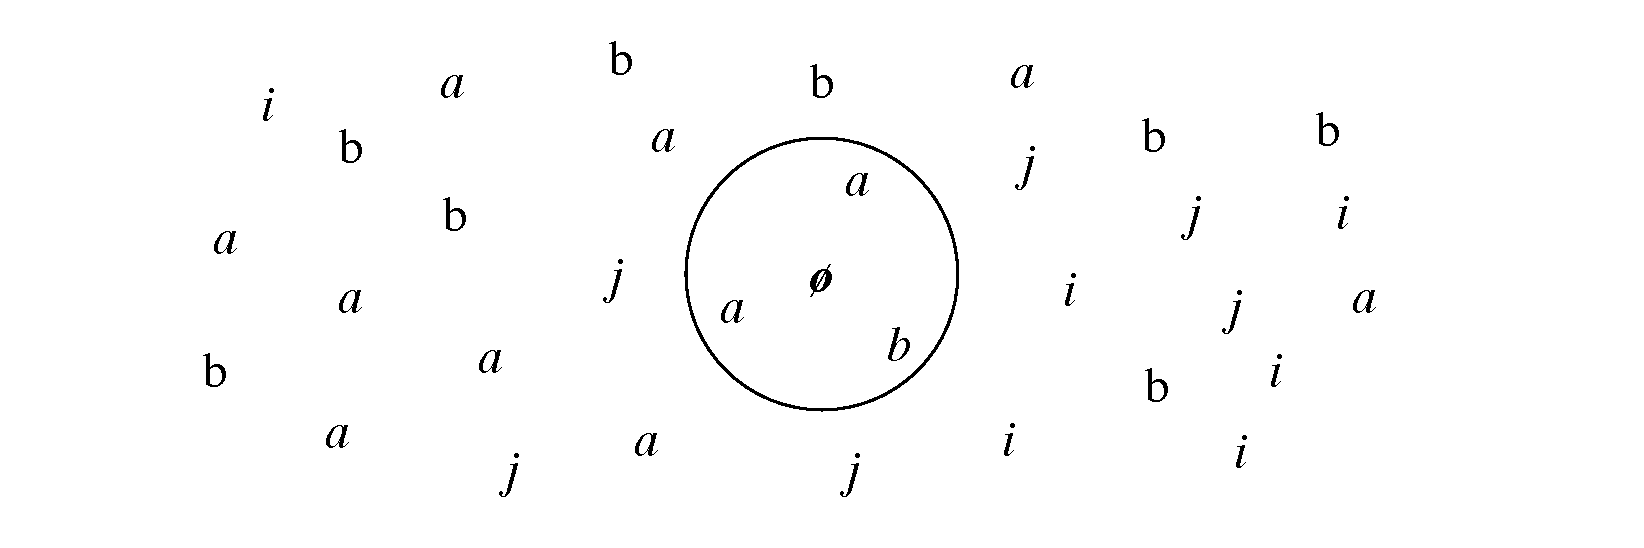
\includegraphics[width=0.8\textwidth]{figures/knn-ex}
  \caption{An example of $k$-nearest neighbors algorithm. An unknown input character \textit{\textbf{\o}} is decided by comparing it with the $k=3$ nearest neighbors. The three nearest neighbors to \textit{\textbf{\o}} are $a$, $a$, and $b$, so in this example \textit{\textbf{\o}}$=a$.} 
  \label{fig:knn}
\end{figure}

The $k$-nearest neighbors algorithm ($k$-NN) is a simple non-parametric classification method \cite[pp. 231-236]{ml}. A training set is embedded in a $n$-dimensional space and used as a prediction model. The model can then predict new data by estimating the shortest distance to the $k$ nearest classes in the $n$-dimensional space, as demonstrated in \autoref{fig:knn}. The unknown character is classified, apparently enough, as the median of the $k$-nearest neighbors classes. 

It is a tangible challenge and computationally heavy to perform classification on high dimensional (i.e. large $n$) data with $k$-NN. Therefore, a dimension reduction algorithm was first applied before the $k$-NN classifier, as described in the next chapter.

\subsubsection{Principal component analysis}
    \label{sec:pca}

A dimension reduction tool is preferable before performing a k-Nearest Neighbor Classifier, as discussed in the previous subsection. In this project, the Principal Component Analysis (PCA) procedure was used for reducing the number of correlated dimensions down to a set of the linearly uncorrelated principal component \cite{pca}. The principal Component Analysis will use too much space to derive in this report. In short, it decomposes the original $n$-dimensional space into $m$ orthogonal dimensions by finding the orthogonal dimensions with the highest variance and computing the variance vector in that dimensions direction. The first dimension will have the highest variance; the second will have the second largest and so on. Numerical estimations show that the optimal condition for the k-Nearest Neighbor Classifier is when PCA is used to reduce the dimension down to $m=\vari{n_pca}$.

The authors spent a substantial  amount of time to make an implementation using $t$-distributed stochastic neighbor embedding \cite{tsne} for easier separation of characters. However, this was not possible as the t-distributed stochastic neighbor embedding algorithm can only visualize trained data, and not transform a test set. If a $t$-distributed stochastic neighbor embedding transform is deactivated, then we believe that the combination of Principal Component analysis,  $t$-distributed stochastic neighbor embedding, and $k$-nearest neighbors algorithm would be interesting to explore.

\subsubsection{Performance of $k$-nearest neighbors algorithm}

To find the best performance of \knn  with PCA, it is useful to implement a search with a nested loop, with a focus on the number $k$ of neighbors and amount of dimension $m$ the data was reduced to. The best performance without implementation was when $k=\vari{n_neighbors}$ and, as mentioned above, $m=\vari{n_pca}$. The best performance was calculated using \autoref{eq:error} and resulted in an error of
\begin{equation}
E_{k\rm NN}=\vari{error} \rm\ \%
\end{equation}
which was higher than the allowed error of this project. We, therefore, continued with an approach based on Linear Support Vector Classifiers, as described in the next section.

\subsection{Linear Support Vector Classifier}

A Linear Support Vector Classifier (LSVC) implemented is a supervised learning model for binary classification \cite{svm}. A Multiclass LSVC was used in this example, which means that the 26 classes are reduced to a set of binary classifications.

Each binary LSVC classification maps the training data's separate categories into points in space, and linearly divide them by an apparent gap. The test data is assigned to the same space and classified based on what side of the division line the data appears. Support Vector Classifiers can perform classify non-linear classification by using kernel tricks, i.e. transforming the data. However, kernel tricks were not applied in this project.

\end{document}